%!TEX root = ../dissertation.tex
\Chapter{Introduction}
% \chapter{Introduction}
\label{introduction}

\newthought{How can we build} theoretically satisfying and practically useful models of the human mind? Historically, there have been two broad approaches. The \emph{rational} approach, exemplified by the work of David Marr \citeyearpar{marr1982vision} and John Anderson \citeyearpar{anderson1990adaptive}, focuses on characterizing the problems people have to solve and the optimal solutions to those problems. Under the assumption that the mind is well adapted to its environment, these optimal solutions then serve as models of cognition. Rational models are satisfying because they tell us \emph{why} the mind works the way it does, and they are useful because they allow us to make generalizable predictions about how people will behave in new environments (i.e., rationally). However, by construction, such models don't explain \emph{how} the mind achieves the rational ideal, and a growing list of systematic cognitive biases \citep{kahneman2011thinking} draws their predictive utility into question. 

In contrast, the \emph{mechanistic} approach focuses on identifying the cognitive processes underlying behavior, often with an emphasis on explaining the behavioral idiosyncrasies that rational models gloss over. This approach can potentially tell us how the mind actually works, and it can produce extremely accurate models. However, lacking the optimality constraint, there is an enormous space of possible mechanistic models, and they typically have free parameters that are tuned for specific experimental setups. We are thus often left wondering why this specific model fit the data best, and whether it would continue to make good predictions in a slightly different context.

Although the rational and mechanistic approaches have traditionally been viewed as conflicting, the past decade has seen a resurgence of an old idea \citep{simon1955behavioral}: rationality can be seen as a property of cognitive mechanisms themselves. Specificially, a cognitive mechanism is rational if it makes optimal use of limited cognitive resources. Going under various names---cognitively bounded rational analysis \citep{howes2009rational}, computational rationality \citep{lewis2014computational,gershman2015computational}, and resource-rational analysis \citep{griffiths2015rational,lieder2020resourcerational} to name a few---this view suggests that we should not expect people to be rational in the traditional sense of taking actions that maximize expected utility \citep{vonneumann1944theory}. Instead, we should expect people to select actions using mental strategies that strike a good tradeoff between the utility of the chosen action and the cogntive cost of making the decision.

But what defines a ``good'' tradeoff between action utility and cognitive cost? And how can we identify mental strategies that achieve such a tradeoff? In this dissertation, I suggest answers to these questions based on a key insight: \emph{a rational mental strategy is one that optimally solves the sequential decision problem posed by one's internal computational environment}. Under this view, cognition is a problem of stringing together a series of basic cognitive operations, or ``computations'', in the service of choosing what to do in the world. An optimal cogntive process strings those basic operations together in such a way that maximizes the difference between the utility of the ultimate behavior and the total cost of all the cognitive operations that support the behavior.


\section{Sequential decisions in the world and the mind}\label{sec:intro-intuition}

To make things concrete, consider the problem facing a delivery robot, illustrated in \figref{fig:sequential-intuition}{a}. Completing the delivery will require visiting a sequence of locations before arriving at the final destination. And at each location, the robot will need to decide where to go next. Thus, the robot faces a \emph{sequential decision problem}. \figref{fig:sequential-intuition}{b} illustrates how this type of problem is often modeled in artificial intelligence research. At each time step, an agent (here, the robot) takes an \emph{action} (e.g., driving forward). This action causes the environment to enter a new \emph{state} (e.g., one where the robot is in a new location). Additionally, the agent receives a \emph{reward}, a number that captures how good or bad the immediate consequences of the action are. The robot's goal is to maximize the total reward received. For example, the delivery robot might receive a large positive reward for reaching the destination and a small negative reward every time it moves (capturing the desire to conserve battery life). After receving the reward and new state, the agent selects another action and the cycle continues.

\begin{figure}[tb]
  \centering
  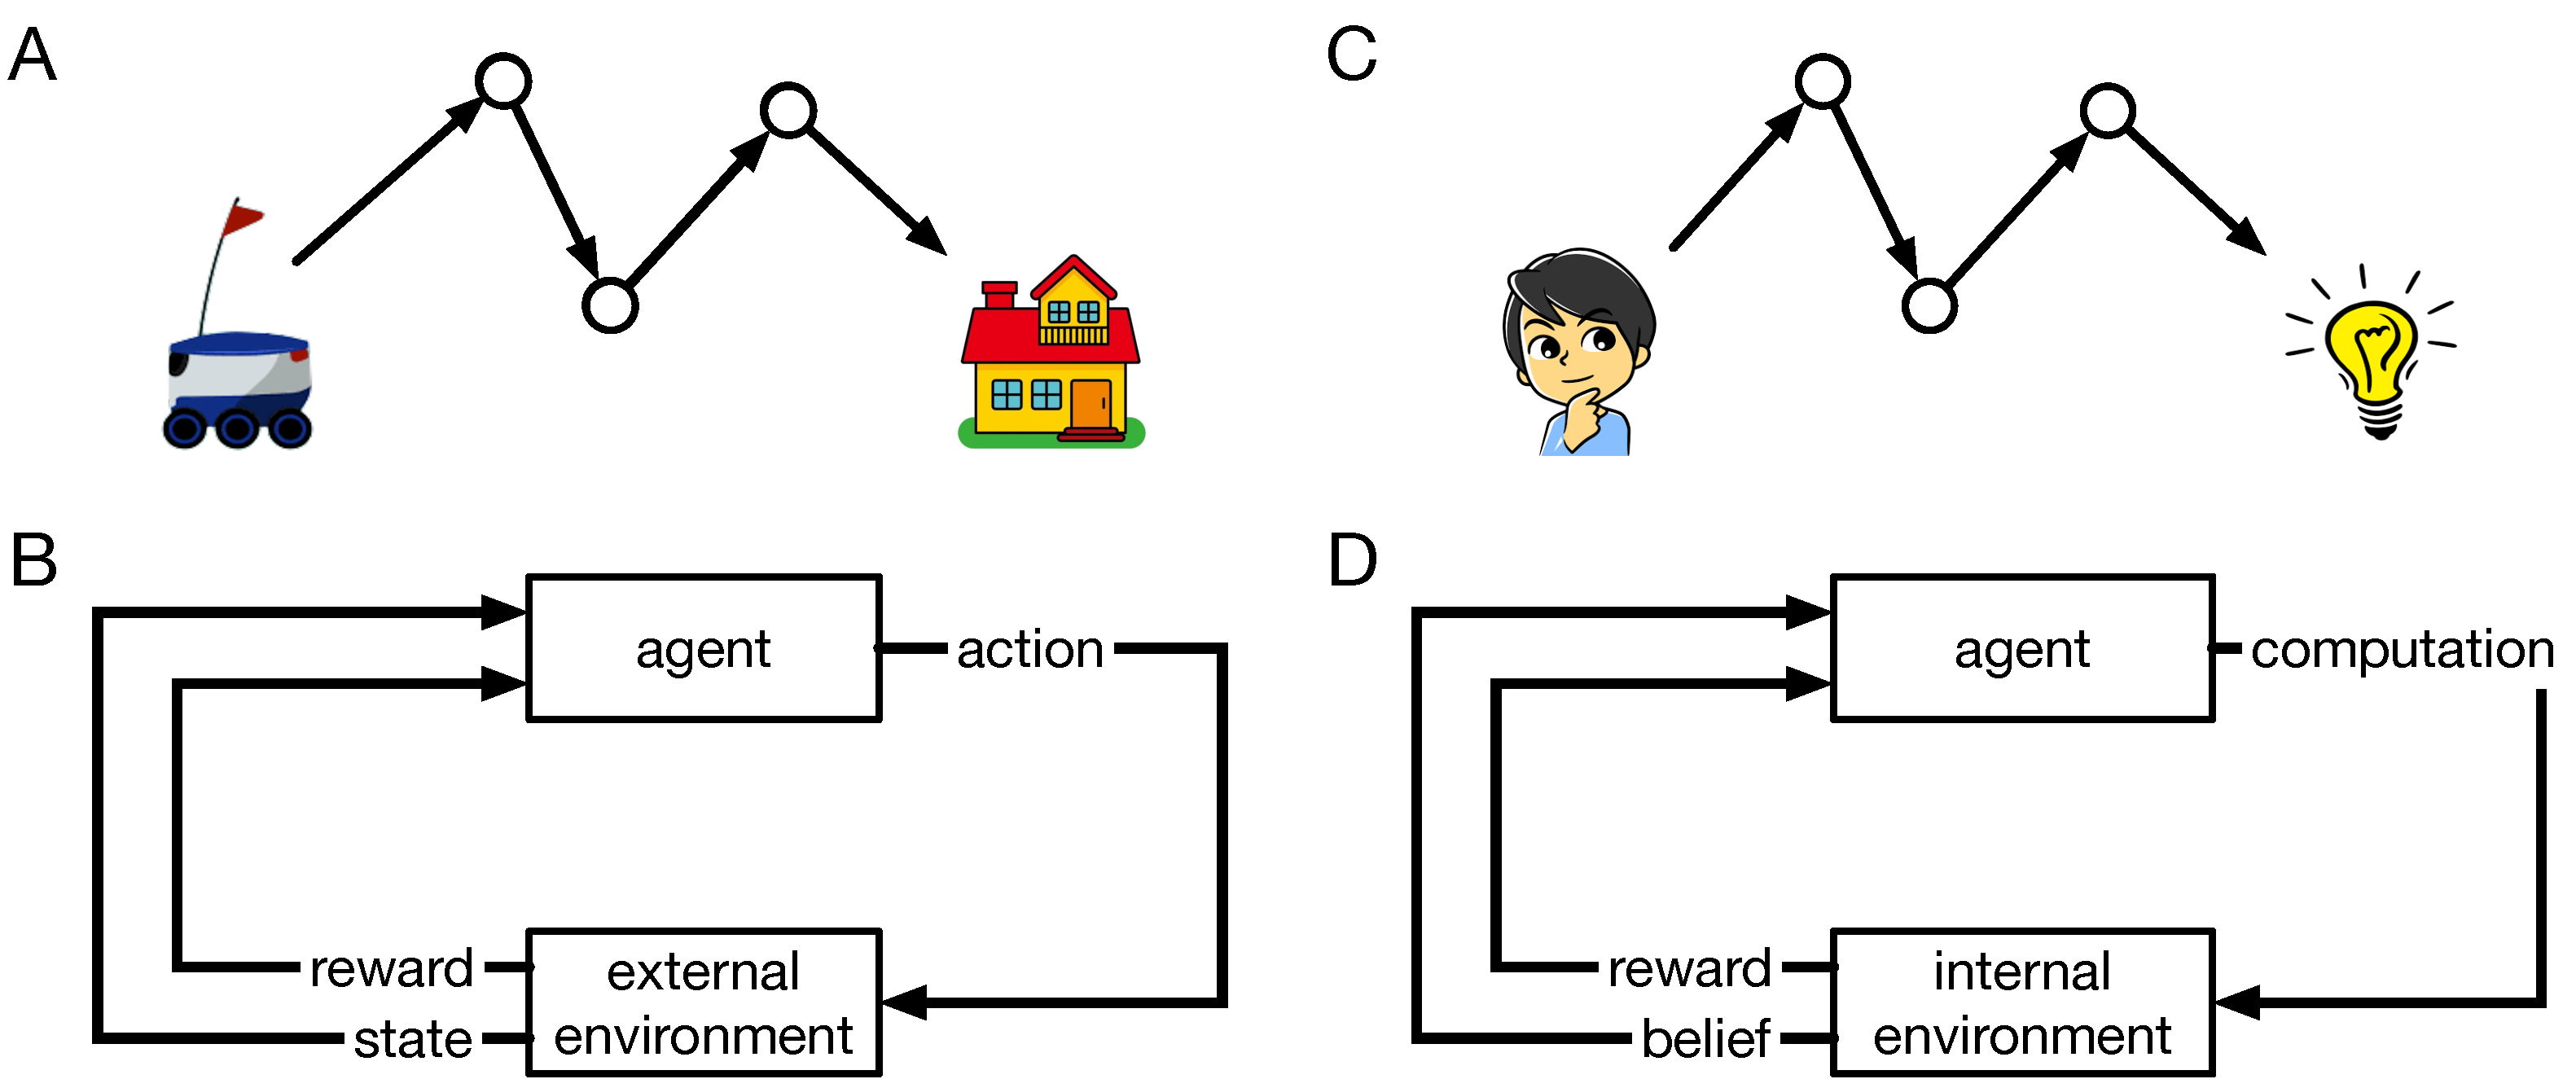
\includegraphics[width=0.9\textwidth]{diagrams/sequential-intuition.pdf}
  \caption{Sequential decision problems posed by external and internal environments.}
  \label{fig:sequential-intuition}
\end{figure}

\figref{fig:sequential-intuition}{c} illustrates a seemingly very different type of situation: a person trying to come up with a solution to a difficult problem. However, as the diagram suggests, the two cases actually share the same basic structure. Both involve an extended interaction between an agent and an environment; but whereas the robot is interacting with an \emph{external} environment, the thinker is interacting with an \emph{internal environment}: their own mind. Just as the robot makes several moves, and visits several locations before reaching the destination, the thinker has several thoughts, and enters several mental states before discovering the solution. Indeed, as illustrated in \figref{fig:sequential-intuition}{d}, this problem can be modeled in precisely the same way as the delivery problem. However, now the actions correspond to computations (thoughts) and the states correspond to beliefs (mental states). Thinking changes one's mental state just as moving changes one's physical state; and it also incurs a cost---at the very least, thinking takes time.

An important property of sequential decision problems is that there is often a dissociation between the short-term reward and the long-term \emph{value} of performing some action. For example, if the robot had the option of simply sitting still, this would incur no cost and would thus be the most rewarding action in a myopic sense. However, the potential for the large reward associated with making a delivery makes paying this cost worthwhile. Thus, moving has value. By the same token, a truly myopic agent (one who only considers immediate rewards) would never do any thinking at all! Thinking only has value insofar as it can inform our future behavior.\footnotemark{}

\footnotetext{Note that, subjectively, thought itself can be rewarding (sometimes intensely so; \citealp{gopnik1998explanation}). However, just as with ``secondary reinforcers'' like money, this is not because thought is inherently valuable, but because it is associated with value. Nevertheless, this association may be deeply engrained, perhaps even genetically so. I return to this question in the conclusion.}

The power of identifying this parallel between external and internal environments is that it allows us to leverage existing knowledge about sequential decision problems (a substantial chunk of AI research) to build rational mechanistic models of cognition. That is, we can apply the same formalisms and algorithms that might help a robot deliver groceries to instead characterize the problem of resource-bounded cognition, and identify cognitive processes that optimally solve that problem.

% \section{The shoulders of giants}

\separator

% \newthought{Our approach builds} on 
\newthought{A long history} of work in artificial intelligence and cognitive science has established the foundations upon which this dissertation builds. Formally, our approach draws heavily on concepts and tools developed in \emph{rational metareasoning}, a subfield of artificial intelligence that aims to construct artificial agents that make effective use of their limited computational resources \citep{russell1991principles,hay2016principles}. Indeed, in many ways, our approach is simply the application of these ideas to understanding human cognition. At the same time, many of these ideas have parallels in cognitive models, and still more can be traced to the period before the boundary between cognitive modeling and artificial intelligence was well-defined. Below, I review these ideas from a psychological perspective, noting the parallel concepts in AI when relevant. Ultimately, I will synthesize these key insights into a formal definition of rational mechanistic models of cognition.

% cognition is \emph{dynamic} (sequential, occuring over time), \emph{bounded} (subject to costs or constraints), and \emph{optimized} (maximizing utility). As illustrated in Table~\ref{tab:comparison}, various combinations of these assumptions are made frequently in models of the mind. However, by capturing all three ideas at once, the current approach has advantages that cannot be achieved with any subset.

\section{Optimal models of cognition}\label{sec:intro-optimal}

What does it mean, formally, for a cognitive model to be rational? Following \citet{anderson1990adaptive}, I formalize rationality in terms of \emph{optimality}. A model of a cognitive process (henceforth just ``a cognitive process'') is optimal if it performs a cognitive function as well as it possibly could. More precisely, an optimal cognitive process is one that produces the maximum value of an \emph{objective function}, out of a set of possible models:
\begin{equation}\label{eq:intro-optimal}
  π^* = \argmax_{π \in \Pi} V(π).
\end{equation}
Here, $V$ (for value) is the objective function, and each $π \in \Pi$ is a possible cognitive model. Defining an optimal cognitive model thus amounts to specifying the function or goal of the cognitive process (through $V$), and the set of possible processes (through $\Pi$).

Perhaps the most fundamental optimal model is expected utility theory, which states that one should select actions that yield the best outcomes in expectation (i.e., on average). Given that the world is in state $w$, the action with maximal expected utility is defined as
\begin{equation}\label{eq:eut}
  a^*_w = \E_{o \mid w, a} U(o).
\end{equation}
Although it was not originally conceptualized in this way, we can think of expected utility theory as an optimal model where the set of possible cognitive processes $\Pi$ contains all possible mappings from world states to actions, and the objective function is defined as
\begin{equation}\label{eq:perfect}
  V(π) = \E_{o \mid \pi} [U(o)] = 
  \E_{w} \left[
    \E_{a \sim \pi(w)} \left[
      \E_{o \mid w, a} U(o)
    \right]
  \right].
\end{equation}
That is, choosing actions according to expected utility theory yields the highest utility outcomes, on average. In rational metareasoning, maximizing $V$, as defined in Equation~\ref{eq:perfect}, is known as \emph{perfect rationality} \citep{russell1997rationality}.\footnote{%
  More precisely, perfect rationality is usually defined in terms of the total utility attained over the agent's lifetime, and it accounts for limits on the information available to the agent (i.e., not knowing $w$). 
  % Equation~\ref{eq:perfect} describes the special case where the agent makes a single choice and has perfect information.
}

Expected utility theory is the foundation of modern (neoclassical) economics, allowing analysts to predict aggregate market behavior by assuming that each individual maximizes their own welfare. But it is so abstract that it initially seems to tell us little about cognition itself. Nevertheless, applying the optimization principle in more constrained domains (perhaps implicitly) has yielded important insights about many areas of cognition, including perception \citep{marr1982vision,knill1996perception,najemnik2005optimal} categorization \citep{anderson1991adaptive,ashby1995categorization,tenenbaum2001generalization}, memory \citep{anderson1989human}, and language \citep{goldwater2009bayesian}.

The power of optimization as a tool for cognitive modeling is that it makes decisions for us. That is, it reduces the amount of flexibility we have when specifying a model. This may sound like an impediment---and indeed, it sometimes feels that way---but it can have enormous benefits. Conceptually, optimal models provide a type of explanation that purely mechanistc models cannot: \emph{teleological explanation}. That is, an optimal model tells us not just how a cognitive process works, but why it works that way. Characterizing a cognitive process as an optimal solution to a problem amounts to identifying that problem as the function of the cognitive process, and sometimes that function is different from what one might have initially assumed (e.g. \citealp{anderson1989human}).

% Conceptually, optimality is a source of intuition. Cognitive processes can be very complex, and simply observing what people do and trying to reason backwards to how they do it can be challenging---especially if we want to understand \emph{why} they do it that way. Exploring optimal solutions, even when they don't explain human behavior especially well, helps us understand the function of cognitive processes, which in turn helps us generate hypotheses about how those processes actually work.
From a statistical perspective, optimality acts as an \emph{inductive bias}. Any given behavioral phenomenon is consistent with countless cognitive models \citep{anderson1978arguments}, but only a small subset of those are optimal. If people are well-adapted to their environment, then all else being equal, the optimal models are more likely to resemble the truth than an arbitrary alternative model. Of course, people are not perfectly adapted to their environment; thus, one can always achieve a more accurate model of a particular phenomenon by abandoning the assumption of optimality. But when data are limited, or we are exploring a domain we know very little about, or we want to generalize our predictions in non-trivial ways, having a constraint that is mostly true can improve our chances of making predictions that are mostly accurate.

Problems arise, however, when optimality isn't even mostly true. And there are many settings where that seems to be the case. To take just one example, recall that according to expected utility theory, one should take actions that yield the highest utility outcomes in expectation. This seems straightforward enough, right? Not for humans. People systematically violate expected utility theory, making choices that cannot be reconciled with any utility function \citep{allais1953comportement,ellsberg1961risk,kahneman1979prospect}. Since then, a major focus in research on human decision-making has been to characterize exactly how and why people violate expected utility theory, for example because they misperceive the probabilities involved \citep{kahneman1979prospect} or don't consider the different actions independently \citep{roe2001multialternative}.

\section{Accounting for constraints}\label{sec:intro-constraints}

Herb Simon \citeyearpar{simon1955behavioral} famously offered a different type of explanation for people's failure to maximize utility: People don't maximize Equation~\ref{eq:perfect} because that's not the problem they're actually faced with. In most real-world problems, there are many actions, and each action could result in many different outcomes. Considering every possible outcome of every possible action each time we are faced with a decision would be paralyzing. Not to mention, the utility of an outcome is itself a complicated thing to evaluate (potentially requiring one to consider the action one would take next given that outcome) and we might not know the exact state of the world (either because the information isn't available or because we simply didn't take note of it). For decisions of the complexity that people face every day, even the largest supercomputers would be completely unable to evaluate expected utilities as in Equation~\ref{eq:eut}. For a person to attempt to do so, using a biological computer that uses less power than an incandescent lightbulb, wouldn't just be hopeless---it would be irrational. 

This notion, that our choices reflect not only the expected utility of their outcomes, but also our limited ability to compute those utilities is called \emph{bounded rationality} \citep{simon1990bounded}. More generally, Simon suggests that human cognition---and the very definition of rational behavior---is shaped by  both ``the structure of task environments and the computational capabilities of the actor'' \citep{simon1990invariants}. By accounting for those constraints as part of the definition of the problem that people have to solve rather than a flaw in the solution, we can continue to apply the rationality principle in cases where computational constraints render perfect rationality (Equation~\ref{eq:perfect}) unattainable.

In modern psychological research, Simon's ideas are reflected in many different ways. One of the most prevalent is the notion of \emph{ecological rationality} \citep{gigerenzer1999simple,goldstein2002models,todd2012ecological}. Ecological rationality is based on the idea that people make decisions using simple, but adaptive heuristics. These heuristics are computationally ``frugal'', meaning that people can actually apply them in the real world, but they result in good decisions most of the time. This is possible because they take advantage of the structure of the problems people face frequently---they are adapted to our ecology. How can we identify such heuristics? Although Gigerenzer and colleagues emphasize the performance of the heuristics they propose (i.e., that they yield correct decisions; \citealp{goldstein2002models}), they explicitly reject the idea of optimizing that performance, suggesting that any form of optimization---\emph{especially} optimization that accounts for cognitive constraints---is ``demonic'' (\citealp{gigerenzer1999simple}; Chapter~1).

An alternative interpretation of Simon's ideas, the one adopted here, is that we can account for the role of cognitive constraints in defining the problems people face without abandoning the methodological tools we use to characterize rational solutions to those problems. Importantly, just as Bayesian models of perception do not claim that people are constantly evaluating multi-dimensional integrals in their heads, identifying optimal solutions to cognitively constrained problems does not imply that people actually perform that optimization. But this raises a new question: how exactly can we account for cognitive constraints within the optimality paradigm?

\citet{lewis2014computational} propose a very natural answer: we can formalize bounded rationality as \emph{bounded optimality}. \citet{horvitz1987reasoning} defines bounded optimality as ``the optimization of computational utility given a set of assumptions about expected problems and constraints on resources'' (compare to Simon's ``structure of task environments'' and  ``computational capabilities''). More formally, \citet{russell1995provably} define bounded optimality as a property of a program, namely that it yields the maximum expected utility when executed on the agent's computational machine, or ``brain'' $B$. We can thus define a bounded optimal cognitive process as
\begin{equation}\label{eq:bo}
  π^*_B = \argmax_{π \in \Pi_B} \E_{o \mid \pi, B} [U(o)],
\end{equation}
where $\Pi_B$ is the set of all cognitive processes that can be executed by brain $B$ and $\E_{o \mid \pi, B} [U(o)]$ is the expected utility of the outcome that results from executing process $\pi$ on brain $B$.

As a definition of rationality for cognitive processes, bounded optimality is perfect in principle, but prohibitive in practice. In principle, it exactly defines the problem that a resource-contrained agent faces: maximizing utility given computational constraints. In pratice, however, it is very difficult to identify bounded optimal cognitive processes. There are two reasons for this. First, it requires optimizing over the set of all cognitive processes a brain could execute. It is not clear how one would even specify this set, let alone find the optimum. Second, bounded optimality is not really a property of cognitive processes---it is a property of \emph{minds}.\footnote{%
  Similarly, in bounded optimality, the objective function is evaluated over the agent's entire lifetime, not a single outcome. This can can be addressed by the notion of long-term value (briefly described in Section~\ref{sec:intro-intuition} and formalized in Chapter~\ref{sec:metamdp}). That is, we can define the utility of an outcome in terms of both the immediate and future rewards it yields.
} A mind serves many cognitive functions, and they all draw on the shared resources of one brain. Thus, we cannot directly apply the principle of bounded optimality to identify the optimal cognitive process for any particular function, because doing so would not account for how the resources used by this process might impact other processes. Taken at face value, bounded optimality prevents us from decomposing the monolithic task of characterizing ``rational cognition'' into a set of more manageable tasks of characterizing specific rational cognitive processes.

Fortunately, these two challenges are not insurmountable, at least if we are willing to make approximations. I address the problem of specifying possible processes in Section~\ref{sec:intro-sequential}, and optimization in Chapter~\ref{sec:metamdp}. The challenge of decomposability is addressed in the next section (in particular, Equation~\ref{eq:resource}).

\section{The cost and value of mental action}\label{sec:intro-cost}

Traditionally, researchers in psychology have taken a different approach to accounting for cognitive constraints. Intuitively, thinking is \emph{effortful}, and so we avoid it for the same reason we avoid carrying heavy groceries \citep{shenhav2017rational}. On the other hand, more thinking generally results in better outcomes. Thus, there is a fundamental trade-off between the utility of the outcomes we experience and the cost of the mental effort we spend to earn those outcomes \citep{kool2018mental}. Critically, however, the optimal point on this trade-off is not always the same. For important decisions with clear factors to consider, thinking a lot is often worthwhile. For unimportant decisions, or ones that are too complex to effectively reason about, the benefit of thinking a lot is unlikely to outweigh the cost.


% One of the key challenges of applying bounded optimality is that the optimization occurs over the agent's entire brain. We use our brains for many different things, and have to decide how much mental resource to allocate to each. When viewed as a single constrained optimization problem, this is intractable, as it requires jointly solving for the optimal cognitive process for all the different problems our brain has to solve.

The idea that a rational cognitive process should allocate different amount of effort in different situations has been formalized in many different ways \citep{shenhav2013expected,anderson1990adaptive,lieder2017strategy}. However, all these different approaches draw on a key insight. The choice of how much effort to allocate is analogous to the choice of which action to take in the world. Accordingly, just as we can define the value of an \emph{action} as the expected utility of the outcome it produces, we can define the value of \emph{cognition} as the expected utility of the outcome it produces, minus cognitive cost. That is,
\begin{equation}\label{eq:evc1}
  V(w, c) = 
    \E_{o \mid w, c} \left[
      U(o)
    \right] - \cost(c),
\end{equation}
where $c$ corresponds to a ``cognitive action''. Simlarly, just as expeceted utility theory defines the optimal physical action to take in each state (Equation~\ref{eq:eut}), we can define the optimal cognitive action to take in each state as
\begin{equation}\label{eq:evc2}
  c^*_w = \argmax_c V(w, c) = \argmax_c \E_{o \mid w, c} U(o) - \cost(c).
\end{equation}
In rational metareasoning, Equation~\ref{eq:evc1} is called the \emph{value of computation} (VOC; \citealp{russell1991principles}).\footnote{%
  More precisely, the VOC is typically defined as the improvement in expected outcome utility compared to if the computation were not executed.}

The content and interpretation of $c$ varies substantially across different instantiations of this general principle. One influential example is the \emph{expected value of control} (EVC; \citealp{shenhav2013expected}). In EVC, $c$ corresponds to a \emph{control signal}, which modulates the behavior of an underlying cognitive process. In the simplest case, the control signal indicates simply how much effort the process exerts. In more complex cases, the control signal can have multiple dimensions, controlling not just the amount but also the nature of cognitive effort exerted \citep{musslick2015computational,grahek2020computational,ritz2021cognitive}.

% \footnote{%
%   Note that we depart from the original definition of EVC \citep{shenhav2013expected} for consistency with the other equations in this section. In the original definition, the utility is defined in terms of the outcome of the process, rather than the behavior iteself. Non-trivially, the outcome was proposed to include the following world state, making EVC a sequential framework. However, most applications of EVC do not actually use this feature, assuming that the utility of the outcome depends only on the behavior in the current trial, as in Equation~\ref{eq:evc1}. One notable exception is the visual attention model in \citet{lieder2018rational}, which employs an early version of the framework proposed here.
% } 

In another instantiation of this principle, $c$ corresponds to a \emph{strategy} for solving a problem. A classic example of this kind of model considers the decision of whether to use a ``model-free'' or ``model-based'' strategy \citep{daw2005uncertaintybased}. Intuitively, a model-free strategy relies on habits or learned associations, while a model-based strategy involves explicit reasoning about the consequences of one's actions. Generally, the model-based system yields better outcomes, but is more costly to execute; people seem to arbitrate between the strategies accordingly \citep{keramati2011speed,kool2017costbenefit}, sometimes using strategies that combine model-free and model-based elements \citep{keramati2016adaptive}. Although this work only makes an intuitive appeal to a cost-benefit tradeoff, \citet{lieder2017strategy} have proposed a model of strategy selection that explicitly optimizes VOC (Equation~\ref{eq:evc1}), showing that it can account for the strategies people use to sort lists and make choices between alternatives that vary on many dimensions.

\subsection{Bounded optimality and metalevel rationality}\label{sec:bound-meta}

Treating the choice of cognitive actions as analogous to the choice of physical actions has yielded important insights into the flexibility with which people allocate mental effort. But as researchers, we now face a difficult choice. On the one hand, bounded optimality (Equation~\ref{eq:bo}) defines the true problem of resource-contrained cognition. But a cost-benefit tradeoff (Equation~\ref{eq:evc2}) is something we can actually work with. Must we choose between principle and practice?

Perhaps not. As defined in Equation~\ref{eq:bo}, bounded optimality poses a constrained optimization problem whose solution is a single cognitive process that solves all the problems the agent might face using a single shared resource, the brain. This is intimidating, to say the least. But it's not the only way to view the problem. Consider another case where an animal must allocate a finite shared resource amongst several different activities: foraging. Rather than allocating mental resources across different cognitive functions, the animal must allocate their time across different patches where food might be found. Initially, this problem seems very challenging because the correct amount of time to allocate to each patch depends on the time allocated to every other patch. But as shown by \citet{charnov1976optimal}, the optimal solution is actually quite simple: stay in a patch as long as the rate of food intake is more than what you could expect to find elsewhere (the average rate of intake in the past). More generally, one should allocate resources to an activity as long as the utility gained from that activity exceeds the \emph{opportunity cost} of not allocating those resources to some other activity. As brilliantly observed by \citet{kurzban2013opportunity}, this principle applies equally to the allocation of cognitive resources. Thinking about any particular thing has an opportunity cost because it means you aren't thinking about something else.

Leveraging the insight that cognition carries an opportunity cost, \citet{lieder2018bounded} showed that we can specify the value of a specific cognitive processes (in a bounded optimal sense) as an additive combination of outcome utility and cognitive cost,
\begin{equation}\label{eq:resource}
  V_B(\pi) = \E_{o \mid \pi,B} [U(o)] - \cost_B(\pi),
\end{equation}
where $\cost_B(π)$ captures the opportunity cost of the resources consumed by $\pi$ on brain $B$.\footnote{%
  \citet{lieder2018bounded} presents a derivation of the opportunity cost in terms of the amount of time that different resources are allocated (each of which is assumed to have some fixed cost). However, more nuanced factors are likely at play, such as the need to be able to quickly re-allocate resources when necessary \citep{musslick2021rationalizing}, and the changing value of other cognitive activities \citep{agrawal2022temporal}.
} This suggests that a cost-benefit tradeoff, such as we see in EVC, could actually be a direct expression of bounded optimality. Perhaps we do not need to make a choice after all!

If this seems too good to be true, that's because it is. To see why, we must ask ourselves: what is the optimal cognitive process in EVC, and what objective function is it optimizing? Initially, we might think of $c^*_w$ as the optimal cognitive process. This makes intuitive sense given that $c$ is often implemented as a parameter that modulates the behavior of an underlying process (like a drift diffusion model, described below; \citealp{musslick2015computational}). But the problem with defining $c^*_w$ as the optimal cognitive process is that we would then have a different objective function for each state. Thich amounts to having a different cognitive model for each condition in an experiment---an undesirable state of affairs. Instead, just as we viewed expected utility theory as an optimal mapping from states to actions, we must view the cognitive process in EVC (and other instantiations of Equation~\ref{eq:evc2}) as a mapping from states to control signals, with the objective function defined analogously to Equation~\ref{eq:perfect}:
\begin{equation}\label{eq:intro-metavalue}
  V(π) = \E_{w} \left[
    \E_{c \sim π(w)} \left[
      \E_{o \mid w, c} U(o) - \cost(c)
    \right]
  \right].
\end{equation}
With some rearrangement, we can make this look more like the bounded optimal objective in Equation~\ref{eq:resource},
\begin{equation}
  V(π) = \E_{o \mid π} \left[
    U(o)
  \right] - \E_{c \mid π} [\cost(c)],
\end{equation}
but there is one critical difference: $\cost_B(\pi)$ is not equal to $\E_{c \mid π} [\cost(c)]$. The former capture the entire cost incurred by the cognitive process. The latter accounts for the cost of the cognitive actions that are selected, but not \emph{the cost of selecting those actions}.

This is the difference between \emph{metalevel rationality} (Equation~\ref{eq:intro-metavalue}) and bounded optimality (Equation~\ref{eq:bo}). Metalevel rationality is defined as selecting computations (cognitive actions) that optimally trade-off utility with computational cost \citep{russell1997rationality}. But, unlike bounded optimality, metalevel rationality is not something that a physically implemented agent can actually achieve; it assumes that computations are selected by a metalevel process, which is separate from the ``object-level'' process that actually performs the computations, and which is not itself subject to any cost or constraints. This assumption is particularly troubling in light of the parallel between selecting computatons and selecting actions (between VOC and expected utility). The observation that people cannot maximize expected utility is what set us on our quest to characterize cognitive constraints, but it has led us right back to the assumption that people are maximizing expected utility! This circularity, sometimes called ``the problem of infinite regress'', is the reason many strategy-selection researchers have abandoned the metacognitive cost-benefit analysis of VOC in favor of models that select strategies through simpler, model-free mechanisms \citep{shrager1998scads,erev2005adaptation,rieskamp2006ssl}.


% Erev & Barron, 2005; Rieskamp & Otto, 2006; Shrager & Siegler, 1998; Siegler, 1988; Siegler & Shrager, 1984).

Is all hope lost? Perhaps not. As suggested by the strategy-selection models just mentioned, one does not have to actually perform a cost-benefit analysis in order to select strategies that effectively balance costs and benefits. Building on this idea, \citet{lieder2017strategy} present a model that explicitly approximates the VOC using learned predictive models of the computational cost and outcome utility that will result from applying a strategy to a particular problem. They call this strategy \emph{metacognitive reinforcement learning}. Although a human being with finite experience may not be able to learn VOC exactly, they may be able to learn a relatively good approximation to VOC, especially for the kinds of metacognitive decisions they encounter frequently. In these cases, their behavior may come close to true metalevel rationality. By the same token bounded optimality and metalevel rationality will actually not be so different in these cases. Thus, going forward, we will use metalevel rationality as an approximation to bounded optimality. I further discuss the validity of this assumptions (and possible improvements on it) in the \todo{conclusion}.
 
\section{Representation, action, and the value of information}\label{sec:intro-info}

Our discussion so far has remained agnostic about an important question: How exactly does cognition influence outcomes? To answer this question, I will draw on another class of models that are used to characterize rational cognition under computational constraints, those based on \emph{information theory}. These models vary widely in their structure and go under different names, including efficient coding \citep{barlow1961possible,stocker2006noise}, rate-distortion theory \citep{sims2016rate}, the free-energy principle \citep{friston2010freeenergy}, and rational inattention \citep{sims2003implications}. Here, I will describe one version of this type of model, which is particularly applicable in decision-making contexts (c.f. \citealp{bhui2021resourcerational}).


The key idea in information-theoretic approaches to bounded rationality is to view cognitive processes as information channels. Specifically, the process consists of two components: an encoder $\pi\enc$ that transforms the world state $w$ into a mental representation $m$, and a decoder $\pi\act$ that chooses an action $a$ based on that representation:
\begin{equation}
  w \xrightarrow[{\displaystyle \pi\enc}]{\text{\tiny encoder}} m 
    \xrightarrow[{\displaystyle \pi\act}]{\text{\tiny decoder}} a
\end{equation}
The agent then receives utility $\Uterm$, a shorthand for the expected outcome utility given the state and selected action, $\E_{o \mid w, \pi\act(m)} U(o)$.

Cognitive constraints are operationalized as an information bottleneck, limiting the amount of information that $m$ can have about $w$, either by making $\pi\enc$ stochastic or by making the number of possible representations less than the number of world states (often both). Different forms of this constraint are possible; a common one is mutual information, which can be intuitively understood as the reduction in uncertainty (entropy, $H$) about the state of the world after observing the mental representation:
\begin{equation}
  I_\pi(m, w) = H(w) - H(w \mid m)
\end{equation}
Intuitively, $I_\pi$ captures the fidelity of the representation, how little information is lost when using $m$ in place of $w$.

To cast this type of model as an optimal cognitive model (in terms of Section~\ref{sec:intro-optimal}), we can take one of two approaches. Rate-distortion models \citep{sims2016rate} typically assume a \emph{capacity limit}. This corresponds to defining $\Pi$ as the set of all encoder-decoder pairs with the constraint that $I_\pi(m, w) < C$, where $C$ is the capacity constraint. In contrast, free-energy \citep{ortega2013thermodynamics} and rational inattention models \citep{caplin2013behavioral} typically assume a continuous \emph{information cost}. This corresponds to letting $\Pi$ include all possible encoder-decoder pairs, but subtracting the information cost from the experienced utilities.\footnote{
  As it turns out, the two approaches are equivalent in some sense. Because mutual information is an expectation over values of $x$ and $w$, one can find a cost-multiplier $λ$ that yields any given mututal information $C$ (the Lagrange multiplier; see \citealp{ortega2013thermodynamics}). Note, however, that the $λ$-to-$C$ conversion depends on the utility function and distribution of $w$. Thus, assuming a fixed $λ$ (rather than fixed $C$) predicts that the information rate can change across experimental conditions (e.g., \citealp{vandenberg2018resourcerational})
} Adopting the continuous-cost convention, the objective function is defined
\begin{equation}\label{eq:intro-info}
  V(π) = \E_w \left[
    \E_{m \sim π\enc(w)} \left[
      \Uterm
    \right]
  \right] - \lambda I_\pi(m, w).
\end{equation}
where $\lambda$ defines the conversion between utility and information cost.
% where $U(w, \pi\act(m))$ is a shorthand for the expected outcome utility, $\E_{o \mid w, \pi\act(m)} U(o)$. 
There are two key ideas to take away from this equation. First, cognitive processes can produce intermediate mental states, which are used to select actions. Second, both the action utility and cost depend on the mental state, and these two forces are in a fundamental conflict. A precise representation of the world allows one to select good actions, but such representations are costly to form.

Rational metareasoning provides another way to think about the mental state. Specifically, we can think about $m$ as a \emph{belief} about the state of the world, $p(w \mid m)$. Assuming that $\pi\act$ is optimal (that is, that it always selects the action with highest expected utility given the representation), we can define the \emph{value of information} \citep{matheson1968economic} in the representation as the expected utility of the action that would be taken based on that information/representation:
\begin{equation}\label{eq:intro-voi}
  % \VOI(m) = \max_a \expectunder{U(w, a)}{w \sim P(w \mid m)}
  \VOI(m) = \E_w \left[\Uterm\right] =
    \max_a \E_{w \mid m} U(w, a)
\end{equation}
A derivation for the second equality is given in Equation~\ref{eq:Rbot-derivation} (see Section~\ref{sec:voi} for more discussion of VOI). Using VOI, we can rewrite the information-theoretic objective function (Equation~\ref{eq:intro-info}) as
\begin{equation}\label{eq:intro-voi}
  V(π) = \E_{m \mid \pi} [\VOI(m)] - I_\pi(m, w).
\end{equation}
Thus, from an information-theoretic standpoint, the value of a cognitive process is the difference between the value of the information it produces and the cost of that information.

The earliest information-theoretic models were applied in perception, particularly how people reduce redundancy in their representation of images \citep{attneave1954informational,barlow1961possible}. A key insight here is that the brain's coding scheme accounts for the statistics of the environment \citep{simoncelli2001natural}. These models can explain phenomena that are puzzling from a purely Bayesian account, such as a systematic bias \emph{away from} the average value of visual stimulus dimension \citep{wei2015bayesian}. This same pattern was later shown in the representation of subjective value \citep{polania2019efficient}. Efficient coding models are also commonly applied in memory \citep{gershman2021rational}. For example, \citet{sims2012ideal} showed that a model that flexibly allocates informational resource across an arbitrary number of items explains human reconstructions better than the classic model with a fixed number of working memory slots. Beyond perception and memory, efficient coding models have been used to explain the exponential shape of people's generalization curves (\citealp{sims2018efficient}; c.f. \citealp{shepard1987universal} and scalar variability in approximate number representation (\citealp{piantadosi2016rational}, c.f. \citealp{fechner1860elemente}).

For the most part, the efficient-coding models discussed above do not emphasize the down-stream function of perception for directing action. In such models $\pi\act(m)$ is simply a guess about the value of $w$, and the $U$ captures the difference between the guess and reality. More recent work has begun to emphasize how our representations are shaped by their use \citep{sims2018efficient}. For example, in visual working memory tasks, people can strategically prioritize more important dimensions of the stimulus \citep{yoo2018strategic} and can also allocate more or less total resource depending on task demands \citep{vandenberg2018resourcerational}. This latter result is interesting because it supports an additive cost like in Equation~\ref{eq:intro-info} over a fixed but costless capacity constraint.

In contrast, economic applications of information theory emphasize the function of representations as supporting decision-making. These models often go under the name \emph{rational inattention}, reflecting the idea that one's mental representation is the result of ignoring features of the world that aren't important to one's decision \citep{sims1998stickiness,caplin2013behavioral}. 
% This idea was initially developed by \citet{sims1998stickiness} to understand why prices don't respond to changing market conditions as quickly as expected-utility-based models predict. List a few findings... 
One interesting result from this literature is that, for the commonly used mutual-information cost function, the optimal cognitive process has exactly one representation for each possible action; that is, there is a one-to-one correspondence between $a$ and $m$. This allows one to eliminate $m$ entirely, yielding a reduced form model in which the cost is simply the mutual information between state and action \citep{matejka2015rational}, as proposed in free-energy based models \citep{friston2010freeenergy,ortega2013thermodynamics}. This reduction is mathematically fascinating, and it can explain some interesting cognitive phenomena such as perseveration \citep{gershman2020origin}. But if our goal is to define rational \emph{mechanistic} models of cognition, we seem to be going backwards. By eliminating the mental representation from the model, we end up with a more sophisticated form of behaviorism, where we attempt to understand a cognitive process simply as a mapping from stimulus to response.

%  Ultimately, the result is a slight variation of the commonly used ``softmax'' model of choice,
% \begin{equation}
%   \pi(a \mid w) \propto \expp{\frac{1}{λ} \cdot (U(w, a) + \alpha_a)}
% \end{equation}
% where $\lambda$ is a scaling constant on the mutual-information cost and $\alpha_a$ captures a default tendency to take action $a$ (the values of $\alpha$ can be determined optimally, being larger for actions that have higher average utility).
% This reduction is mathematically fascinating, and it provides a useful extension of the standard softmax model by accounting for the habitual tendency to take actions that are usually good. 
% However, if our goal is to define rational \emph{mechanistic} models of cognition, we seem to be going backwards. By eliminating the mental representation from the model, we end up with a more sophisticated form of behaviorism, where we attempt to understand a cognitive process simply as a mapping from stimulus to response.

% Importantly, however, this reduction can only be applied under the assumption that all conceivable representational mappings are actually possible. By making stronger, psychologically motivated, assumptions about the form of the cognitive process (the mapping), we can still glean interesting cognitive insights. For example, \citet{bhui2018decision} use 

% Thus, information-theoretic models are well-suited for explaining how we represent the world and why we behave somewhat randomly. But they are perhaps less ideal for understanding the mechanisms that generate those representations or yield that randomness.
% Nor is it clear how to apply these models in cases where the cost is not naturally cast in terms restricted information flow.

\section{The sequential nature of thought}\label{sec:intro-sequential}

Thus far, I have described models that rationally select mental actions, and models that form mental representations to inform the actions they take in the world. These are key ingredients for a rational mechanistic model of cognition, but something is still missing. All the models we've discussed so far treat the problem of rational metacognitive control as a \emph{static} problem (or a sequence of independent static problems). That is, they consider the selection of a single mental action or a single mental state.\footnote{%
  It is perhaps unfair to call EVC or strategy selection ``static'', given that the control signals often parameterizes a dynamic evidence accumulation process and the strategies are correspond to multi-step algorithms. More precisely, it is the rational metacognitive component of these models that is static. I discuss this further at the end of this section.
} But cognition is not static; it is \emph{dynamic}. Cognitive processes are not defined by solitary representations or operations; they consist of sequences of mental states, and the mental actions that produce and transform them.

The fact that cognitive processes are sequential, in the sense that they occur over time rather than all at once, is self-evident. Thus, sequentiality is a common feature of mechanistic models of cognition. One widely used class of sequential models are \emph{evidence accumulation} models (also called ``sequential sampling models''), such as the drift diffusion model (DDM; \citealp{ratcliff1978theory}), leaky competing accumulators \citep{usher2001time}, and decision by sampling \citep{stewart2006decision}. According to these models, decision making involves accumulating noisy evidence in favor of each possible choice until the evidence for one choice is sufficiently greater than the evidence for the other(s). That is, the cognitive process can be understood as a sequence of operations, each of which accumulates a small amount of evidence. In their simplest form, there is only one type of operation; these models can explain not only the choices we make (including when we make mistakes), but also how long it takes to make those choices. More complex evidence accumulation models take into account the possibility of attending to different sources of information, such as different options \citep{krajbich2010visual} or attributes \citep{russo1983strategies}; these models can account for (if not predict) additional data such as what we look at when making a decisision, and they can account for systematic deviations from expected utility \citep{busemeyer2019cognitive}.
% For example, these models predict that easier decisions will be made both more consitently and more quickly, and that mistakes will be faster than correct choices.

Another important class of dynamic models, \emph{cognitive architectures}, aims to capture a more diverse range of mental activities, beyond simply accumulating more evidence. Cognitive architectures, most notably ACT-R \citep{anderson1996act} and SOAR \citep{laird1987soar}, explicitly model individual cognitive operations such as perceptually encoding a stimulus, recalling information from memory, and transforming symbolic reprenstations the world. These models can trace their intellectual roots to the infancy of artificial intelligence research \citep{newell1956logic}, where the discovery that digital computers could solve complex problems by breaking them down into a sequence of very simple operations led to the hypothesis that a similar principle might underlie human intelligence \citep{newell1958elements,newell1972human}. The core assumption of these models is that all cognitive processes can be broken down into \emph{elementary information processes} \citep{simon1979information,posner1982information,chase1978elementary}, or simply, ``cognitive operations''.

How can we formally define sequentiality? Intuitively, a sequential cogntive process can be decomposed into two components: the cognitive architecture and the strategy for using that architecture. The cognitive architecture consists of the set of operations that can be performed $\C$, the set of (mental) states the system can be in $\M$, and the relationship between the two: the way that cognitive operations affect mental state. We can define this relationship with a \emph{transition function} $T$, such that
\begin{equation}
  m_{t+1} \sim T(m_t, c_t, w).
\end{equation}
That is, at each time point, the next mental state is (stochastically) determined by the previous mental state, the operation thas was executed, and the state of the world. Together, $\C$, $\M$, and $T$ can be seen as a formalization of the agent's ``computational capabilities'' \citep{simon1955behavioral}, or the architecture on which a program is executed \citep{russell1995provably}.

The second component of a sequential cognitive process is the strategy for using the architecture. Drawing on the models discussed in Section~\ref{sec:intro-cost}, we will formalize this strategy in terms of a policy for choosing mental actions. However, there, we assumed that the agent selected cognitive operations based on the state of the world. To capture the fact that the right operation to execute depends on one's mental state (and also the fact that the world state is often not directly accessible), we can instead assume that the operation is selected based on the current mental state, that is,
\begin{equation}\label{eq:intro-sequential}
   c_t \sim \pi(m_t).
\end{equation}
Note that I use the notation $\pi$ to refer specifically to the strategic component of the cognitive process. This reflects the assumption that the agent has control over their strategy, but not their cognitive architecture---that is, only the strategy $\pi$ can be optimized. Note, however, that on a developmental and evolutionary timescale, the architecture itself may itself be optimized (subject, of course, to some form of constraint). I discuss this further in the \todo{conclusion}.

Before we continue, it is important to clarify how the type of sequentiality described in this section (and the proposed framework) differs from the models described in Section~\ref{sec:cost}. Those models were actually not static in a strict sense, as the mental actions under consideration themselves corresponded to dynamic cognitive processes (e.g. decision-making strategies). Critically, however, those proceses were not themselves subject to rational metacognitive control. In contrast, in the proposed framework, we will assume that the entire cognitive process is optimized; that is, we will consider cognitive processes that are not just sequential and optimal, but \emph{sequentially optimal}.\footnote{%
  Note also that the original definition of EVC \citep{shenhav2013expected} defines outcome utility in terms of EVC at the next time step, making EVC a sequentially optimal framework in principle. In practice, however, most applications of EVC do not actually use this feature, assuming that the utility of the outcome depends only on the behavior in the current trial. One notable exception is the visual attention model in \citet{lieder2018rational}, which employs an early version of the framework proposed here.
}




% To make things concrete, we will illustrate how a simple cognitive process can be formalized in this way. Specifically, we will use the DDM. In this model, noisy evidence in favor of one choice vs. another is accumulated until a threshold level of evidence is reached. Here, the mental state is the total accumulated evidence and the cognitive operations correspond to either taking another sample or choosing one of the options. The transition function is defined
% \begin{equation}
%   m_{t+1} = m_t + ε  \quad\text{where}\quad ε \sim \Normal(0, σ^2).
% \end{equation}
% That is, at each time point, the next 

% and the policy $π$ is defined
% \begin{equation}
%   \pi(m) = \begin{cases}
%     \text{choose A} &\text{if } m > b  \\
%     \text{choose B} &\text{if } m < -b  \\
%     \text{draw sample} &\text{if } -b ≤ m ≤ b
%   \end{cases}
% \end{equation}
% where $b$ is the threshold.

% Formalizing a cognitive process in this way provides a natural way to define the cost of executing a strategy, as the sum of the cost of each operation it executes:
% \begin{equation}\label{eq:intro-cost}
%   \cost(π) = \E_w \left[
%     \E_{\cseq \mid \pi} \left[
%       \sum_t^N \cost(c_t)
%     \right]
%   \right].
% \end{equation}
% where $\cseq = (c_1, c_2, \ldots, c_N)$ is a sequence of cognition operations.
% This may look like kicking the can down the road, but defining the cost of a strategy as the sum cost of all the operations it executes represents real progress. This is because operations are much simpler objects than strategies, and so their cost can be more easily estimated \citep{donders1969speed}. Even without empirical measurement, very simple assumptions (e.g. that all operations have the same cost) can yield useful predictions. For example, using this assumption, \citet{payne1988adaptive} analyzed the cost and expected action utility of a set of ten possible decision strategies, finding that people used strategies that struck good cost-benefit tradeoffs, adapting their choice of strategy to time constraints and the structure of the decision problems.

% On the other hand, formalizing cognitive processes as mappings from mental states to cognitive operations poses considerable challenges. Many models have a very large space of possible mental states, and we need to specify which cognitive operation is executed in each one. If there are $M$ possible mental states and $C$ possible operations, there are $C^M$ possible mappings. If $M$ is large (and it often is), this results in a huge space of possible cognitive processes. Searching this entire space is effectively impossible. Payne et al. circumvented this problem by manually specifying a small set of candidate strategies (mappings). But how can we be sure that this set includes the strategies people use, or that achieve the best cost-benefit trade-offs? Indeed, as shown by \citet{howes2009rational}, failing to consider all the possible strategies can yield incorrect conclusions about which cognitive architectures are consistent with a given pattern of behavioral data. But as the set of strategies grows, more and more architectures become consistent with the data. As Howes et al. convincingly argued, adopting additional constraints---specifically, the assumption of optimality---may be necessary to distinguish between candidate architectures.

% Constructing dynamic models poses a substantial challenge, however, particularly when there are many different elementary operations. Because any number of cognitive operations can be executed at any time, one must not only specify the set of operations and their effects, but also a strategy for how the operations are chosen \citep{payne1988adaptive}. In practice this is often done in an ad hoc manner (c.f., \citealp{howes2009rational}).

% \begin{equation}
%   \cost(π) = \expect{\sum_t \cost(c_t)}{c_t \sim π}
% \end{equation}

% \pagebreak

\section{Optimal sequential models of resource-bounded cognition}\label{sec:intro-final}

\definecolor{optimal}{HTML}{e41a1c}
\colorlet{simon}{SchoolColor}
\definecolor{utility}{HTML}{4daf4a}
\definecolor{info}{HTML}{377eb8}
\definecolor{sequential}{HTML}{7B2FB0}
% \definecolor{cost}{HTML}{D4609A}


\newcommand{\hl}[2]{%
  {\color{#1!90!black} #2}
}

\newcommand{\specialitem}[2]{%
  \item[%
    {\color{#1} \textbf{#2}}%
  ]
}

The literature reviewed above highlights just a sliver of the progress we have made in the project of building rational mechanistic models of cognition. Each of these research programs has yielded important insights into the structure that rational mechanistic models should have. In this dissertation, I attempt to synthesize key insights from each of these programs into a framework for constructing rational mechanistic models that are (approximately) bounded optimal and sequential:
%
\begin{enumerate}
  \specialitem{optimal}{1} An optimal cognitive process is one that maximizes an objective function (Section~\ref{sec:intro-optimal}).
  %
  \specialitem{simon}{2} Cognitive processes are shaped by the structure of both the external environment and the agents computational capabilities (Section~\ref{sec:intro-constraints}).
  %
  \specialitem{utility}{3} The value of a mental action depends on both the utility of the outcome it produces and the opportunity cost of performing that action (Section~\ref{sec:intro-cost}).
  %
  \specialitem{info}{4} The behavior produced by a cognitive process is mediated by the mental state it produces (Section~\ref{sec:intro-info}).
  %
  \specialitem{sequential}{5} A cognitive process can be broken down into a sequence of elementary cognitive operations (Section~\ref{sec:intro-sequential}).
\end{enumerate}%
Combining these ideas, yields the following definition of an optimal sequential cognitive process:
%
\begin{equation}\label{eq:intro-master}
  π^* = \hl{optimal}{\argmax_{π}}\ 
    \E \left[
      \hl{utility}{U}(\hl{simon}{w}, \hl{info}{\pi\act(m_N)})
      \ - \sum_{t=1}^N \hl{utility}{\cost(c_t)}
      % \ - \hl{sequential}{\sum_t} \hl{utility}{\cost(c_t)}
      \ \middle\vert\ \hl{sequential}{c_t \sim \pi(m_t)},
      \ \hl{simon}{m_{t+1} \sim T(m_t, c_t, w)}
    \right]
\end{equation}
That is, the optimal cognitive process is a way of selecting cognitive operations that yields a mental state from which high utility actions can be taken, while at the same time minimizing the total cost of those operations. The equation is certainly complex; but as the tacky coloring reveals, none of these ideas are new.

The idea combine these ideas is not entirely new either. For example, there is a long history of modeling optimal speed-accuracy tradeoffs using evidence accumulation models, like the ones described in the previous section. \citet{bogacz2006physics} showed that the drift diffusion model is the continous limit of the \emph{sequential probability ratio test} (SPRT; \citealp{wald1945sequential}), an optimal stopping rule for collecting evidence about binary hypotheses (c.f. \citealp{gold2002banburismus}). For any given level of evidence coherence (problem difficulty), there is some fixed decision threshold that maximizes the reward rate; this is equivalent to maximizing a linear combination of choice utility and cost under certain assumptions.\footnote{
  For a given decision problem, there is some time cost such that maximizing the reward rate will also maximize the reward minus cost \citep{wald1948optimum,drugowitsch2012cost}. However, this mapping will vary for problems of different difficulty or stakes. For example, increasing the payoffs for correct and incorrect decisions by a multiplicative factor does not change the optimal reward-rate strategy, but it does change the optimal utility-minus-cost strategy.
}. However, this analysis relies on a number of assumptions that rarely hold in the real world. Explicitly modeling evidence accumulation as a sequential decision problem has allowed researchers to characterize optimal stopping rules in more complex cases \citep{drugowitsch2012cost,fudenberg2018speed,tajima2019optimal}. Going beyond the decision of \emph{when} to accumulate evidence, the question of \emph{where} to accumulate evidence has been addressed in optimal models of visual search, which characterize the optimal sequence of eye movments one should make when searching for a target image amongst distractors \citep{butko2008ipomdp,acharya2017human,hoppe2019multistep}. Optimal sequential models have also been applied to characterize rational strategies for using working memory \citep{oreilly2006making,todd2008learning,suchow2016deciding}, episodic memory \citep{lu2022neural}, and long-term memory \citep{zhang2022optimal}. I further discuss these related approaches in \conclusion.

This dissertation helps to unify the work reviewed above by providing a common framework for modeling many different kinds of cognitive processes. Furthermore, by explicitly connecting to both the rational metareasoning literature and the more general reinforcement learning literature, we build bridges with which we can import both mathematical tools and psychological concepts. The former allows us to identify optimal strategies for architectures that are too complex for standard methods (e.g., Section~\ref{sec:bmps}). The latter allows us to apply what we know about how people learn to act adaptively in the world to understand how they learn to think adaptively using their own cognitive architectures (through ``metacognitive reinforcement learning'', discussed further in \conclusion).

In the next chapter, I present the formal framework that makes this possible:  \emph{metalevel Markov decision processes}. This framework formalizes the problem of sequential interaction with a cognitive architecture, the problem for which Equation~\ref{eq:intro-master} is the optimal solution.
